\documentclass{article}

\usepackage{enumerate}
\usepackage{amsmath,amsthm,amssymb}
\usepackage{tikz}
\usepackage{pgfplots}
\usepackage{multicol}
\usepackage{tcolorbox}
%\pgfplotsset{compat=newest}

\newcommand{\greybox}[2]{\begin{tcolorbox}\textbf{#1:}\\ {#2}\end{tcolorbox}}


\usepackage[margin=0.5in]{geometry}

\begin{document}

\noindent \textbf{Name:}\underline{\hspace{2in}} \hfill \textbf{Logs and Exponentials}

\greybox{Sum Rules}{
  \vspace{-1em}
  \begin{enumerate}
    \item $\cos(\theta_1 + \theta_2) = \cos(\theta_1) \cdot \cos(\theta_2) - \sin(\theta_1) \cdot \sin(\theta_2)$
    \item $\sin(\theta_1 + \theta_2) = \cos(\theta_1) \cdot \sin(\theta_2) + \sin(\theta_1) \cdot \cos(\theta_2)$
    \end{enumerate}
  }

\begin{enumerate}
\item Find ``double angle formulas'' for sine and cosine. (Hint: write $2 \theta = \theta + \theta$ and apply sum rules.)
\greybox{Double Angle Rules}{
  \vspace{-1em}
  \begin{enumerate}
    \item $\cos(2 \theta ) = $ \\ \\
    \item $\sin(2\theta) =$ \\ \\
    \end{enumerate}
  }
  \vspace{1in}
\item Find ``difference rules'' for sine and cosine. (Hint: write $\theta_1 - \theta_2$ as $\theta_1 + (-\theta_2)$ and use the sum rules. Simplify using even/odd functions.)
  \greybox{Difference Rules Rules}{
  \vspace{-1em}
  \begin{enumerate}
    \item $\cos(\theta_1 - \theta_2) = $ \\ \\
    \item $\sin(\theta_1 - \theta_2) =$ \\ \\
    \end{enumerate}
  }
  \vspace{1in}
\item Find $\sin(15^\circ)$ and $\cos(15^\circ)$. (Hint: write $15^\circ$ as the difference of two angles whose trig values we already know.)
  \newpage
\item Find $\sin(\arcsin(0.2) + \arcsin(0.4))$
  \vspace{2in}
\item Find $\cos(\arcsin(0.2) + \arccos(0.4))$
  \vspace{2in}
\item Find the value of $x$ in the following triangle. (Hint: find $\overline{NT}$ and $\overline{AT}$.)
  \begin{center}
    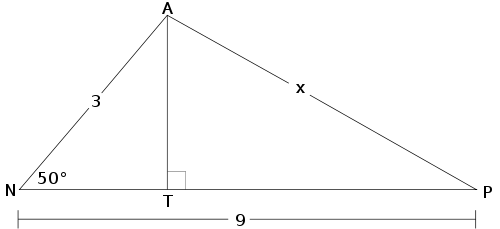
\includegraphics[scale=0.5]{triangle_trig.png}
  \end{center}
\end{enumerate}

\end{document}
